\documentclass{standalone} % DO NOT CHANGE THIS
\usepackage{tikz}
\usepackage[utf8]{inputenc}
\usepackage{graphicx}
\usepackage{times}
\usepackage{amssymb}
\usetikzlibrary[arrows.meta, positioning,math, calc, shapes.geometric,intersections, fit, backgrounds, decorations.pathmorphing]

\begin{document}

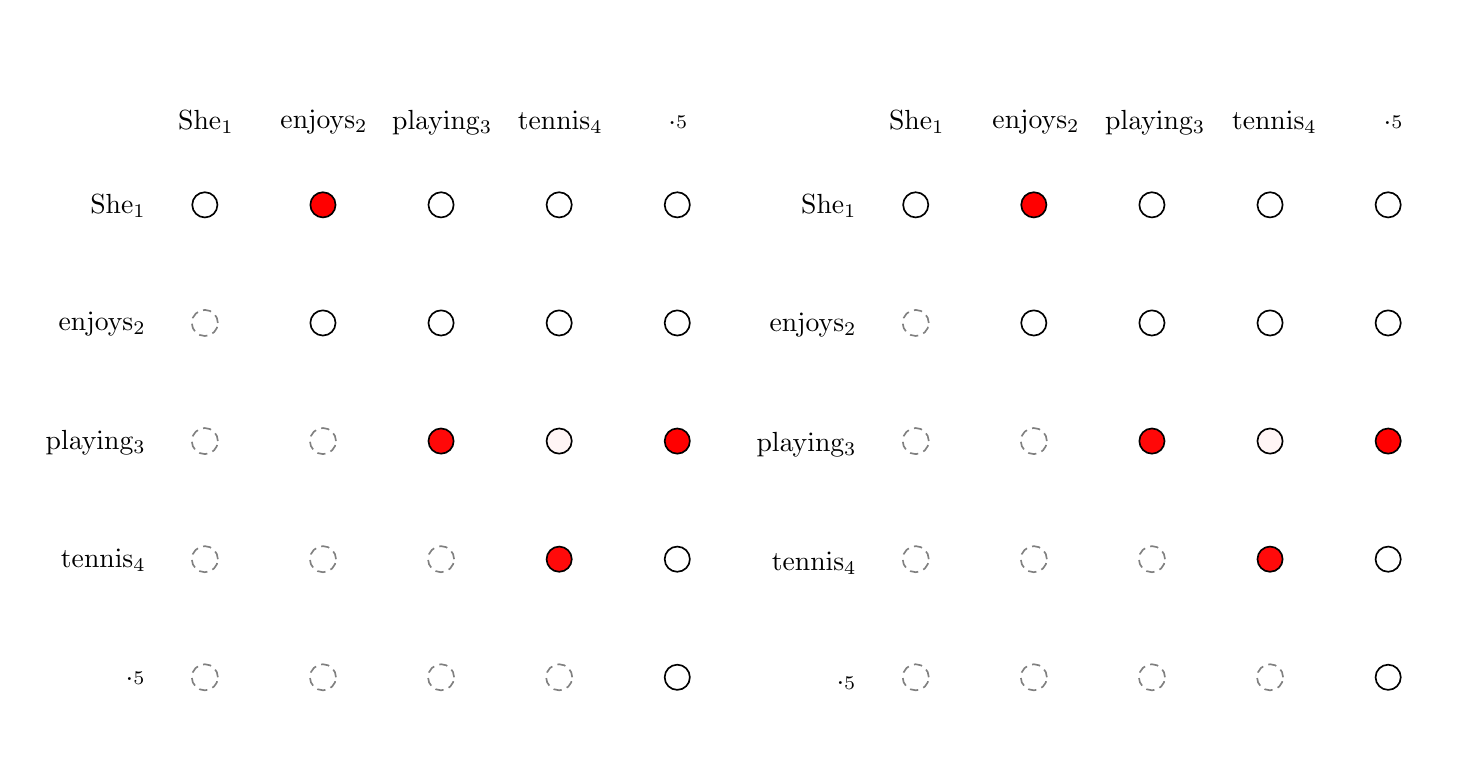
\begin{tikzpicture}[
    word/.style={
            minimum width=1.5cm,
            minimum height=1.5cm,
            inner sep=0pt,
            text width=1.5cm,
            % draw=black
        },
    red filled/.style={
            fill={rgb,255:red,238; green,63; blue,77},
        },
    blue filled/.style={
            fill={rgb,255:red,17; green,101; blue,154},,
        },
    red connect/.style={
            draw={rgb,255:red,238; green,63; blue,77},
            shorten >= 1pt,
            shorten <= 1pt,
            semithick
        },
    blue connect/.style={
            draw={rgb,255:red,17; green,101; blue,154},
            shorten >= 1pt,
            shorten <= 1pt,
            semithick
        },
    connect/.style={
            shorten >= -0.5pt,
            shorten <= 1pt,
        },
    dep arrow/.style={
    arrows={-Latex[round,length=6pt,width=3.5pt]},
    semithick
    },
    ]
    \centering

    \node [word] [anchor=south west] (w00) {};
    \node [word] [anchor=north, align=right] (w001) at ($(w00.south) - (0, 1.5cm*0)$) {She$_1$};
    \node [word] [anchor=north, align=right] (w002) at ($(w00.south) - (0, 1.5cm*1)$) {enjoys$_2$};
    \node [word] [anchor=north, align=right] (w003) at ($(w00.south) - (0, 1.5cm*2)$) {playing$_3$};
    \node [word] [anchor=north, align=right] (w004) at ($(w00.south) - (0, 1.5cm*3)$) {tennis$_4$};
    \node [word] [anchor=north, align=right] (w005) at ($(w00.south) - (0, 1.5cm*4)$) {.$_5$};
    \node [word] [anchor=south west, text centered, minimum height=0.6cm] (w010) at ($(w00.south east) + (1.5cm*0, 0)$) {She$_1$};
    \node [word] [anchor=south west, text centered, minimum height=0.6cm] (w020) at ($(w00.south east) + (1.5cm*1, 0)$) {enjoys$_2$};
    \node [word] [anchor=south west, text centered, minimum height=0.6cm] (w030) at ($(w00.south east) + (1.5cm*2, 0)$) {playing$_3$};
    \node [word] [anchor=south west, text centered, minimum height=0.6cm] (w040) at ($(w00.south east) + (1.5cm*3, 0)$) {tennis$_4$};
    \node [word] [anchor=south west, text centered, minimum height=0.6cm] (w050) at ($(w00.south east) + (1.5cm*4, 0)$) {.$_5$};

    \foreach \y [count=\n] in {
            {   0, 100,   0,   0,   0},
            {   0,   0,   0,   0,   0},
            { 100,   0,  97,   4, 100},
            {   0,   0,   0,  96,   0},
            {   0,   0,   3,   0,   0},
        } {
            \foreach \x [count=\m] in \y {
                \ifnum\m<\n
                    \node [circle,draw=gray, densely dashed ,semithick,minimum size=0.32cm]  (w\x\y) at ($(w00.base) + (1.5cm*\m,-1.5cm*\n)$) {};
                \else
                    \node [circle,draw=black,fill=red!\x, semithick,inner sep=0pt,minimum size=0.32cm]  (w\x\y) at ($(w00.base) + (1.5cm*\m,-1.5cm*\n)$) {};
                \fi
            }
        }


    \node [word] [anchor=south west] (w10) at (w050.south east) {};
    \node [word] [anchor=north, align=right] (w101) at (w10.south) {She$_1$};
    \node [word] [anchor=north, align=right] (w102) at (w101.south) {enjoys$_2$};
    \node [word] [anchor=north, align=right] (w103) at (w102.south) {playing$_3$};
    \node [word] [anchor=north, align=right] (w104) at (w103.south) {tennis$_4$};
    \node [word] [anchor=north, align=right] (w105) at (w104.south) {.$_5$};
    \node [word] [anchor=south west, text centered, minimum height=0.6cm] (w110) at (w10.south east) {She$_1$};
    \node [word] [anchor=west, text centered, minimum height=0.6cm] (w120) at (w110.east) {enjoys$_2$};
    \node [word] [anchor=west, text centered, minimum height=0.6cm] (w130) at (w120.east) {playing$_3$};
    \node [word] [anchor=west, text centered, minimum height=0.6cm] (w140) at (w130.east) {tennis$_4$};
    \node [word] [anchor=west, text centered, minimum height=0.6cm] (w150) at (w140.east) {.$_5$};

    \foreach \y [count=\n] in {
            {   0, 100,   0,   0,   0},
            {   0,   0,   0,   0,   0},
            { 100,   0,  97,   4, 100},
            {   0,   0,   0,  96,   0},
            {   0,   0,   3,   0,   0},
        } {
            \foreach \x [count=\m] in \y {
                \ifnum\m<\n
                    \node [circle,draw=gray, densely dashed ,semithick,minimum size=0.32cm]  (w\x\y) at ($(w10.base) + (1.5cm*\m,-1.5cm*\n)$) {};
                \else
                    \node [circle,draw=black,fill=red!\x, semithick,inner sep=0pt,minimum size=0.32cm]  (w\x\y) at ($(w10.base) + (1.5cm*\m,-1.5cm*\n)$) {};
                \fi
            }
        }

\end{tikzpicture}
\end{document}

